\documentclass[a4paper,12pt]{article}
\usepackage{amsmath}
\usepackage{graphicx}
\graphicspath{ {images/} }
\usepackage[utf8]{inputenc}
\usepackage[english]{babel}
\usepackage[document]{ragged2e}
 \usepackage{mathpazo}

 
\begin{document}\begin{flushleft}\newline \textbf{6.819 PSET 5}
\newline \textbf{10/19/2017}
\end{flushleft}
\newline \begin{center}\textbf{ISAAC KONTOMAH}
\end{center}
\begin{flushleft}
\newline \emph{Collaborators: Devin Morgan , Khamoya Ikhofua,Afika Nyati , Suman Nepal , Abishkar Chhetri}
\end{flushleft}

\newline \emph{\textbf{1. Wiener Filter In Frequency Domain}}
\newline $Y=H \star X + N $
\newline $P_{XX}[u,v]=|X_{F}[u,v]|^{2}|$
$,P_{HH}[u,v]=|H_{F}[u,v]|^{2}|$
\newline $$\epsilon^{2}=E(| \hat{X_{F}}[u,v]-X_{F}[u,v]^{2} |)=\sum_{u,v}|\hat{X_{F}}[u,v]-{X_{F}}[u,v]|^{2}$$
\newline $$=\sum_{u,v}|X_{F}[u,v]-G.Y|^{2} $$
\newline $$=\sum_{u,v}|X_{F}-G.Y|^{2} $$ , but $Y=HX_{F}+N$
\newline $$=\sum_{u,v}|X_{F}-G.(HX_{F}+N)|^{2} $$ 
\newline $$=\sum_{u,v}[X_{F}(1-GH) \mp GN]^{2} $$ 
\newline $$=\sum_{u,v}[X_{F}(1-GH) - GN]^{2} $$ 
\newline $$=\sum_{u,v}[X(1-GH) - GN][X^{\star}(1-GH)^{\star}-G^{\star}N^{\star}]$$ 
\newline $$=\sum_{u,v}[XX^{\star}(1-GH)(1-GH^{\star}) - X(1-GH)G^{\star}N^{\star}-GNX^{\star}(1-GH)^{\star}+GNN^{\star}G^{\star}]$$ 
\newline $$=\sum_{u,v}[X_{F}[u,v]^{2}-X_{F}[u,v]^{2}GH-X_{F}[u,v]^{2}G^{\star}H^{\star}+X_{F}[u,v]^{2}H_{XX}^{\star}GG^{\star}+GNN^{\star}G^{\star}]$$ 
\newline but $P_{XX}[u,v]=|X_{F}[u,v]|^{2}|$ and $P_{HH}[u,v]=|H_{F}[u,v]|^{2}|$
$$=\sum_{u,v}[P_{XX}-P_{XX}GH-P_{XX}G^{\star}H^{\star}+P_{XX}H_{XX}^{\star}GG^{\star}+GNN^{\star}G^{\star}]$$ 
\newline $$=\sum_{u,v}[P_{XX}-P_{XX}GH-P_{XX}G^{\star}H^{\star}+P_{XX}H_{XX}G]^{2}$$ 
\newline $$=\sum_{u,v}[P_{XX}-P_{XX}GH-P_{XX}G^{\star}H^{\star}+P_{XX}H_{XX}|G|^{2}+|G|^{2}\sigma^{2}]$$ 
\newline but $|G|^{2}=G_{R}^{2}+G_{im}^{2}$
\newline Hence , $$\epsilon^{2}=\sum_{u,v}[P_{XX}-P_{GG}(G_{R}+jG_{im})(H_{R}+H_{im})-P_{XX}G^{\star}(H_{R}-jH_{im})^{\star}+P_{XX}H_{XX}(G_{R}^{2}+G_{im}^{2})$$ \\ 
\newline $$+G^{2}(G_{R}^{2}+G_{im}^{2})]$$
\newline $\frac{\partial \epsilon^{2}}{\partial G_{R}}=-P_{GG}H-P_{XX}H^{\star}+P_{XX}H_{XX}-2GR+2\sigma^{2}G_{R}^{2}$
\newline $G_{R}=\frac{H_{F}^{real}P_{XX}}{P_{XX}P_{HH}+\sigma^{2}}$
\newline $G_{im}=\frac{H_{F}^{im}P_{XX}}{P_{XX}P_{HH}+|N_{F}[u,v]|^{2}}$
\newline$G_{F}^{Real}[u,v]=\frac{H_{F}^{real}P_{XX}}{P_{XX}P_{HH}+|N_{F}[u,v]|^{2}}$
\newline$G_{F}^{Complex}[u,v]=\frac{H_{F}^{im}P_{XX}}{P_{XX}P_{HH}+|N_{F}[u,v]|^{2}}$


\newline \emph{\textbf{2. EigenFaces}}

\begin{document}
\newline First Image using 1st eigenvector 

 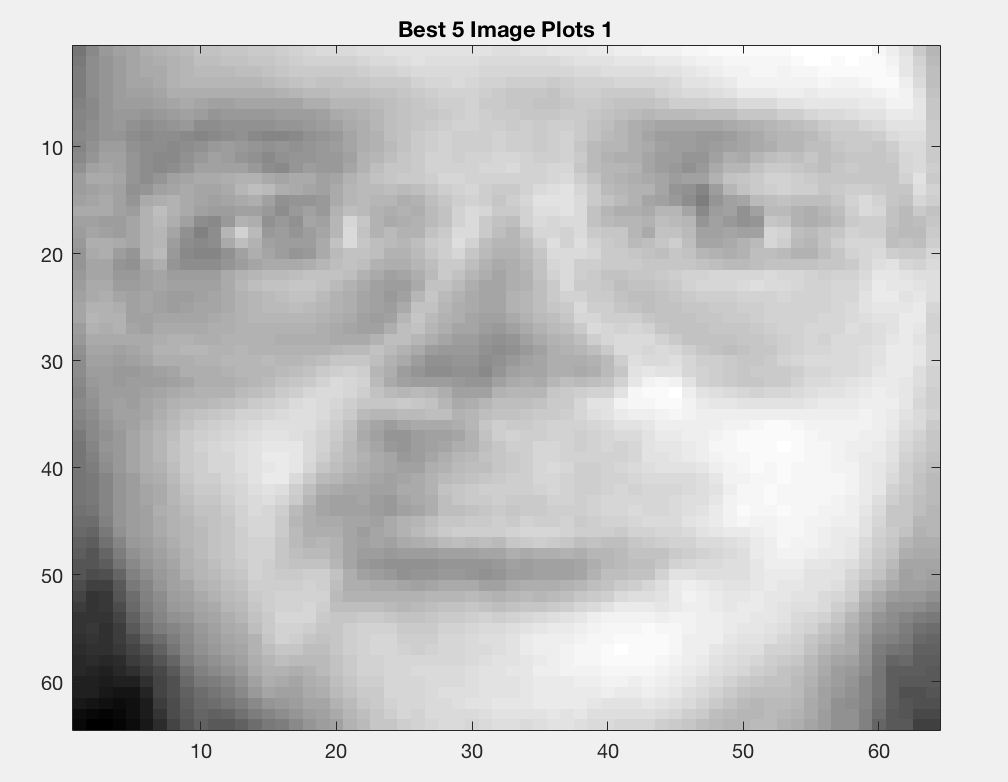
\includegraphics[width=4cm,height=4cm]{plot1.jpg}
 
 First Image
\end{figure}
\begin{document}
\newline Second Image using second eigenvector

 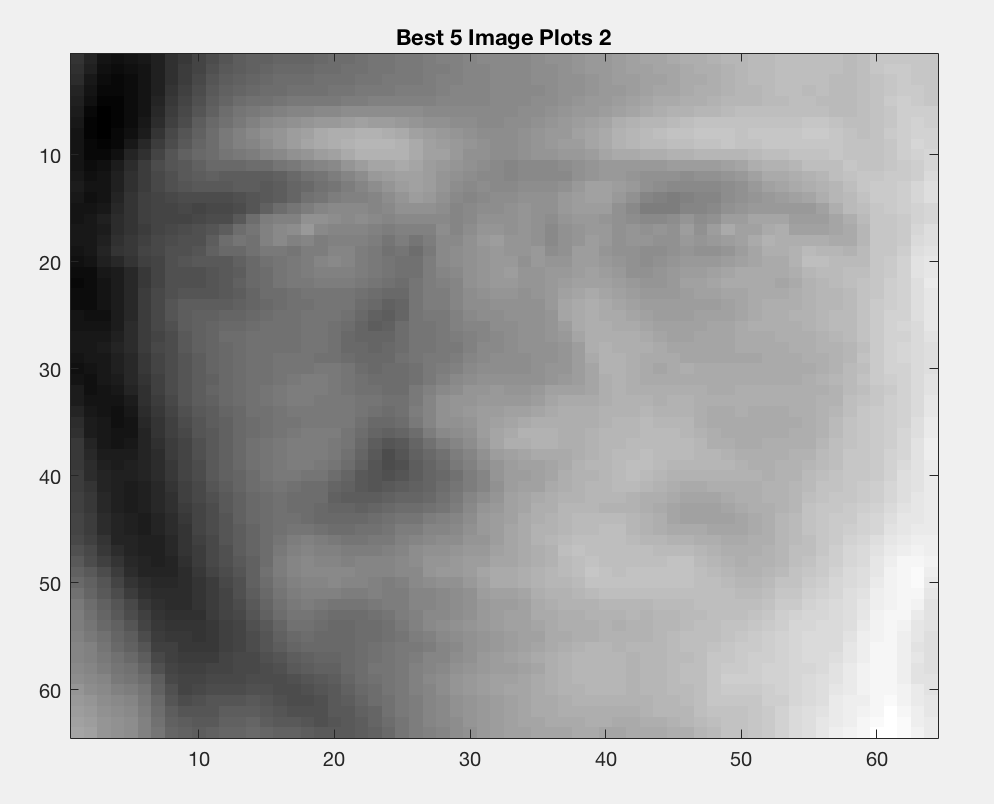
\includegraphics[width=4cm,height=4cm]{plot2.jpg}
 
 Second Image
\end{figure}
\begin{document}
\newline Third Image using third eigenvector

 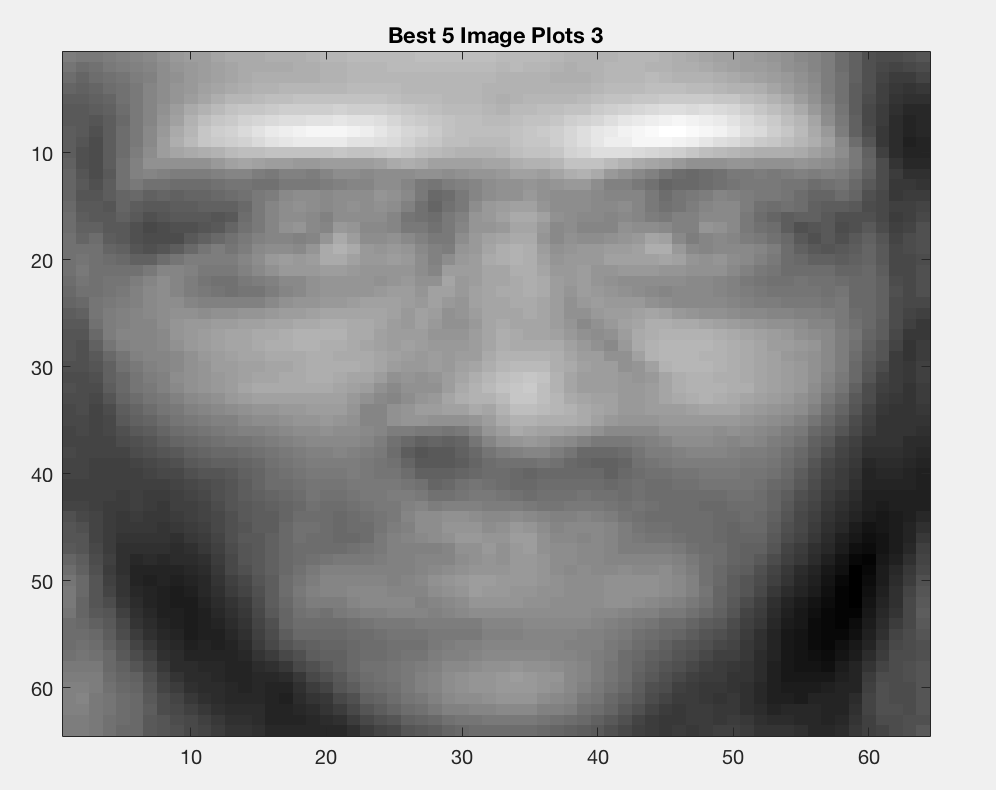
\includegraphics[width=4cm,height=4cm]{plot3.jpg}
 
 Third Image
\end{figure}
\begin{document}
\newline 4th Image using 4th eigenvector

 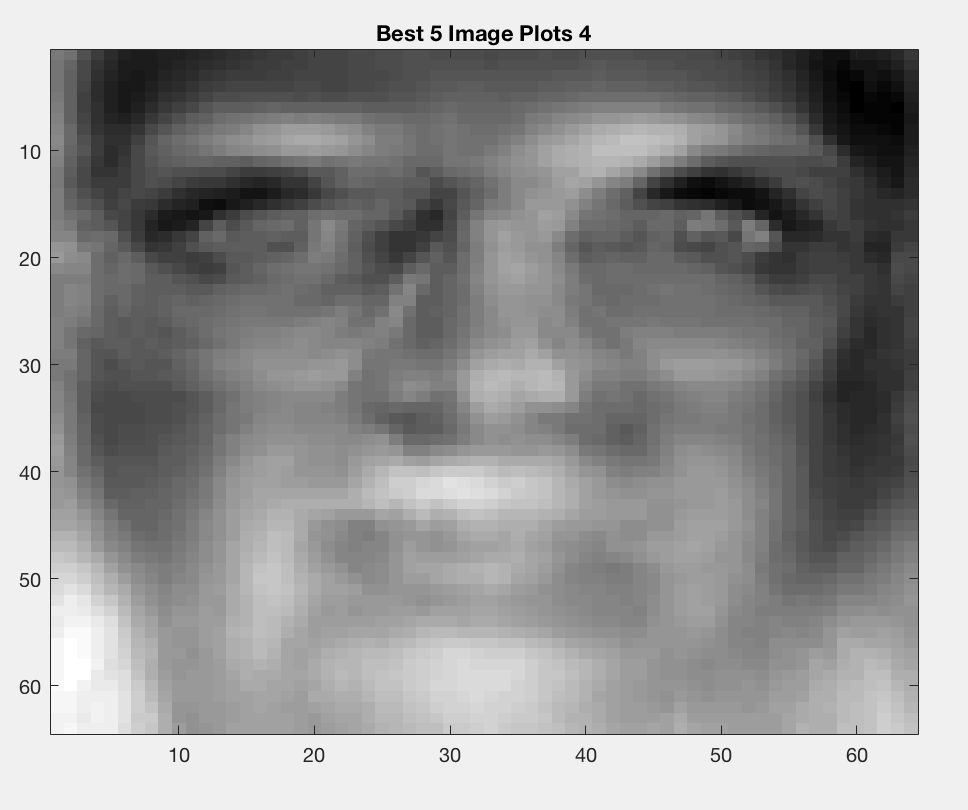
\includegraphics[width=4cm,height=4cm]{plot4.jpg}
 
 4th Image
\end{figure}

\begin{document}
\newline 5th Image using 5th eigenvector

 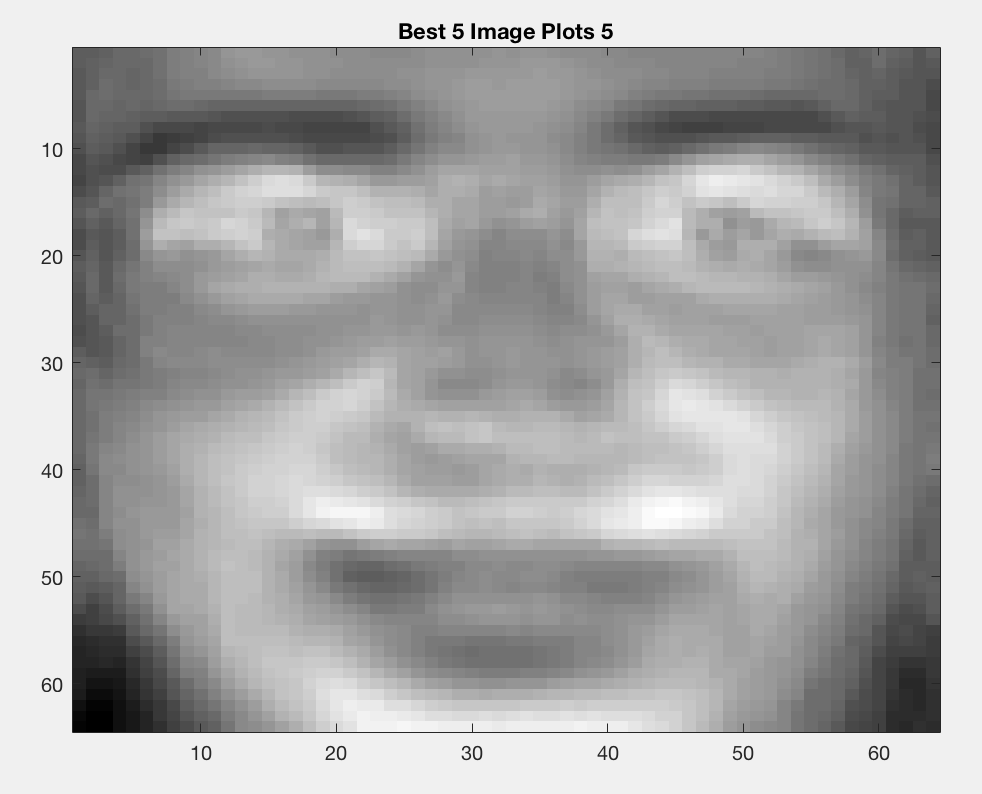
\includegraphics[width=4cm,height=4cm]{plot5.jpg}
 
 5th Image
\end{figure}

\begin{document}
\newline Reconstruction Image using best $20$ eigenvectors

 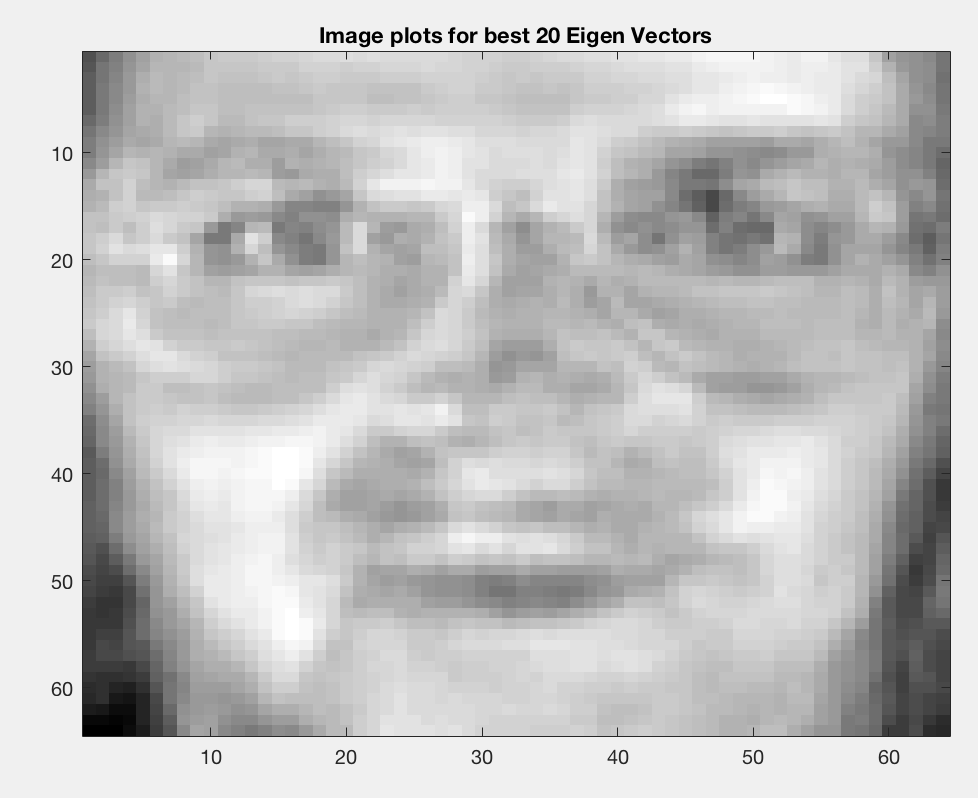
\includegraphics[width=4cm,height=4cm]{best_20.jpg}
 
 Reconstruction Image
\end{figure}
\newline \emph{\textbf{Choosing Best 5 Images}}
\newline \emph{PCA Reconstruction}=$PC Scores.EigenVectors^{T}+$ $Mean$ 
\newline From this equation , it can be seen that the quality of the reconstruction image is directly proportional to the quality of the eigen vectors , hence the higher eigen vector values will produce better images , so I chose the $k$ largest eigenvector values as the basis.
\end{document}